\vspace{-0.2in}
\section{Introduction}\label{intro}

\vspace{-0.1in}


%While automated tools can find recurring patterns, outliers, and other anomalies in the data, the accuracy of such data-intensive tasks heavily hinges on the {\em quality of the underlying data itself}.
 Human workers or crowd can  be  used  as  a  building  block  in data-intensive applications, especially for acquiring and  validating data. One such fundamental crowdsourcing task is {\em labeling}, where a human worker is asked to provide one or multiple labels for the underlying observation. A plethora of applications in cyber human system directly benefit from such efforts, where the objective is to design automated classification/prediction algorithms but require {\em labeled data} for that. Even though human intelligence provides substantial benefit to computation, incorporating humans in the computational loop incurs {\em additional burden} - it becomes time-consuming, monetarily expensive, or both in such cyber-human systems. 
 
Active learning principles~\cite{al1,al2} are proposed to optimize system-centric criteria in classification problems, by employing human workers judiciously only for a few tasks. When crowd is involved in data acquisition, additional challenges emerge: (1) contribution from crowd is potentially noisy, (ii) to ensure  higher engagement and productivity, one has to understand {\em worker-centric criteria}~\cite{martin2014being}, such as, {\em worker skill, motivation}, that are referred to as {\em human factors} in the literature~\cite{amer2016human,hf1,motiv1,motiv2}. In a hybrid human-machine computational environment, an opportunity exists in {\em laying a scientific foundation for predictive analytics} that combines system-centric optimization derived from active learning~\cite{al1,al2} principles and worker-centric optimization through human factors modeling. 

\begin{figure}
\centering
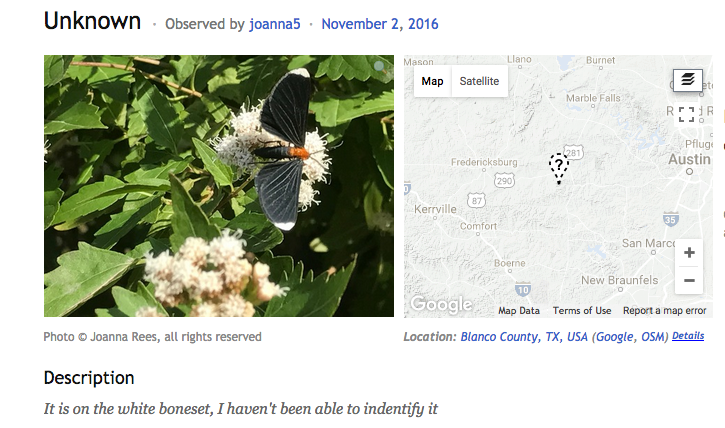
\includegraphics[scale=0.3]{submissions/senjuti/figures/unknown.png}
\caption{\label{fig:unknown} \small Unidentified Species at iNaturalist Website}
\end{figure} 

Imagine that a computational ecologist wants to design a binary classifier~\cite{garzon2006predicting} that accurately predicts the presence or the absence of species given environmental covariates (such as geographical coordinates, elevation, soil type, average precipitation, etc). In order to learn the classifier, the ecologist needs annotated data (i.e., identify the presence or absence of a species in a given location). Indeed, as shown in Figure~\ref{fig:unknown}, there exists unidentified species at large-scale citizen science based platforms like iNaturalist that are to be crowdsourced to be labeled by their registered workers. While doing that, we however need to find the most ``suitable'' worker  taking into account worker-centric criteria, such as, her geographic distance from the observation location, her expertise and/or motivation to identify insects, by considering her past activities/tasks. The goal is to focus on applications, where the workers (e.g., registered citizen scientists of iNaturalist) are involved in completing tasks that are repetitive in characteristics and do not evolve much over the time. We propose to develop an {\em optimized human-machine intelligence framework for such cyber-human systems for single and multi-label classification problems~\cite{single1,multi0} through active learning}. 
%In particular, we are interested to investigate tasks that involve human workers to provide (collecting or acquiring) and validate single and multiple labels. 

Our effort will be investigate and adapt existing {\em active learning techniques for a few well known supervised algorithms for single-label and multi-label classification in the context of crowdsourcing, especially considering worker-centric optimization through human factors modeling}. The general idea behind active learning is to select the instances that are likely to be most informative. Then the selected instances are annotated by human, and the computation loop is repeated.  Our innovations lie in appropriately capturing these two fundamental yet complementary facets in a single optimization function, performing systematic investigation to these problems and designing innovative solutions. 


%An active learner may pose queries, to be labeled by an oracle (e.g., a human annotator), or fetch the raw unlabeled data itself. We however shall focus on the multiple annotator scenario where an oracle, who knows the ground truth, no longer exists; instead, multiple labelers (workers), with varying expertise, are available for querying.

%Generally speaking, crowd-based data
%sourcing is invoked to obtain data, to aggregate and/or fuse data, to process data, or, more
%directly, to develop dedicated applications or solutions over the sourced data.


%
\begin{example}\label{ex1}
{\bf Motivating Example:} 
The iNaturalist platform contains photo vouchered independently verified species occurrence records by the citizen scientists across the world and is one of the fastest growing source of contributions to the global biodiversity information facility. We focus on such platforms, where tasks are repetitive in nature, do not change over the time, and one can retain all the past tasks undertaken by the registered workers (citizen scientists). A computational ecologist makes use of such platforms to develop species distribution models using environmental covariates. Thus, she aims to design a crowdsourcing effort to judiciously obtain single and/or multiple label(s) to annotate some of the unidentified images (refer to Figure~\ref{fig:unknown}). A single label acquisition is about identifying the insect (which will then be augmented with the location information), whereas, multiple labels will require identifying the Kingdom, Phylum, Class, Order, Sub-Order, Family, Sub-family of the insect in the image. 

%Imagine an ecologist wants a binary classifier that accurately predicts the presence or absence of species given environmental covariates (such as geographical coordinates, elevation, soil type, average precipitation, etc). In order to learn the classifier, the ecologist needs annotated data (i.e., species labeled as present or absent). To get such labels, the ecologist designs a citizen science effort.
%
%{\bf Tasks:} There are different types of data collection activities involved that are construed as tasks in this settings. 
%a. initial observations must be collected to measure the covariates and the presence or absence of the species. \\
%b. more observation must be collected (especially for the sites without any training data) to validate the effectiveness of the model.\\
%c. after the initial model is built, more observation may be needed to improve the quality of prediction. \\

%
%\vspace{-0.1in}
%\begin{example}\label{ex2}
%{\bf Multi-labels acquisition:} From the species images available at iNaturalist many of which are indeed unidentified (Figure~\ref{fig:unknown}), an ecologist aims to  design a crowdsourcing effort to judiciously obtain multiple label(s) to annotate some of those images (e.g., Kingdom, Phylum, Class, Order, Sub-Order, Family, Sub-family of the insect in the image). From the collected labels, she would design a classifier that predicts multiple class labels of an insect, given environmental covariates.
%\end{example}
%\vspace{-0.1in}

%A citizen science website (such as, iNaturalist) contains thousands of photo-vouchered, independently verified species (such as, birds) occurrence records.

For these examples, label acquisition involves human workers. On the other hand, domain expert may not have many human workers at her disposal who are qualified for the task - even if there are workers, they may not be {\em motivated} to undertake these tasks. Furthermore, workers may even have constraints (e.g., only likes to watch birds, can not travel more than $25$ miles from her location). Therefore, which task(s) are to be selected and assigned to which worker(s) remain to be a problem.
\end{example}
%the involved domain expert  may not have all the training samples - leading to poor accuracy of the classification task. The volunteers (workers) may have to be involved to collect more training data.
 
%Not only citizen science, the aforementioned scenarios arise in other domains (e.g., web or  healthcare applications)  and computational tasks (e.g., prediction, search, recommendation, data cleaning). 

{\bf Desirable properties:} To generalize, the above scenarios call out for the following desirable characteristics: (1) An ``activized'' label acquisition is desirable - i.e., acquire more data only when it optimizes the underlying computational task considering system-centric criteria. (2) At the same time, select workers and assign tasks to enable {\em worker-centric optimization}. (3) We argue the necessity of studying these two facets together as a single {\em optimization problem}, as a staged solution (first select sub-tasks based on active learning, then assign those to the workers to enable worker-centric optimization) may be inadequate, as tasks selected by active learning techniques may end up having a very low worker-centric optimization, resulting in poor outcome overall.

{\bf High level approach:} (1) We propose {\em worker-centric optimization by characterizing human factors} in the crowdsourcing context by adapting well-known theories of behavioral psychology~\cite{hf1,motiv1,motiv2}. (2) We propose system-centric optimization  by adapting a set of well-known {\em active learning techniques} for supervised algorithms \cite{al1,al2,al-survey,qbc1,al-clus1,al-clus2,al-clus3,al-clus4,multi0,multi1,multi2,multi3} and augment them by combining worker-centric optimization through human factors modeling. (3) We propose systematic investigations on how the two {\em aforementioned optimization problems could be combined} and propose effective solutions. 

Additionally, we will design both retrospective as well as prospective studies. We will perform these evaluations using publicly available citizen science datasets.


{\bf Novelties:} To the best of our knowledge, no existing work has studied what we propose. The closest  related works for active learning through crowdsourcing are for single label acquisition~\cite{active-learning-cs1, active-learning-cs2, mozafari2014scaling,corleone,clamshell}. Worker-centric optimization is not considered there. Active learning research for multi-labels 
remains in a rather nascent state~\cite{multi0,multi1,multi2,multi3}. These aforementioned studies do not investigate the problem in the context of crowdsourcing. Therefore, the necessity of worker-centric optimization does not even arise there. Our designed prototypes on iNaturslist platform will bear a long-lasting effect to understand global bio-diversity.


%selection of task (i.e., what data to acquire) and workers have to be judicious and must account for the combined goal of system optimization and worker-centric optimization considering human factors.

%In fact, we argue that the aforementioned two challenges must not be studied individually and must be investigated together as a principled optimization problem.

%Some workers may have preference to perform {\em diverse tasks}, whereas, others may continue to repeat {\em similar tasks}. Therefore, the next challenge is {\em to be effectively compose tasks for the available workers by appropriately characterizing tasks.}




%Solving this optimization problem is an arduous challenge to a domain expert. Ideally, the domain expert should be able to choose some declarative constructs to specify the aforementioned task using  a SQL-like query and she should be relieved from the burden of any further complexity.  Therefore, the final challenge is {\em how to support declarative constructs for task composition}.







%``off-the-shelf'' classification and clustering algorithms involving crowd} that serve as the core technique of a myriad of computational problems, such as,  entity resolution. 


%The combination of human-machine intelligence can be deployed in a variety of domains and holds enormous potential to contribute to a myriad of scientific, business, and computational problems. For example, hundreds of thousands of volunteers have classified craters on planetary surfaces \\ (http://clickworkers.arc.nasa.gov), deciphered scanned text (ReCaptcha),  discovered new galaxies (Galaxyzoo), or collected species observation data for biodiversity (ebird, iNaturalist). Similarly, commercial and business strategies  have also gained success through human intelligence, with examples ranging from crowdsourcing t-shirt designs (Threadless) to research and development (Innocentive). 
\vspace{-0.1in}
\subsection{Research Objectives} 
\vspace{-0.1in}
Our long term vision is to optimize knowledge discovery processes for cyber-human systems. We are interested in designing effective solutions and support both worker and system criteria  through active learning and human factors modeling. The research proposed here puts us on track to achieving this vision by addressing a first series of concrete challenges on a very important application domain.

%This project has two primary research thrusts:

%\begin{enumerate}
\smallbreak \noindent {\bf (1) Optimized {\em single-label acquisition} involving crowd}: In this research aim, we strive to propose optimization guided hybrid human-machine algorithms considering active learning for single label acquisition. Active learning is popular in {\em single label supervised algorithms}, where the key idea is that a machine learning algorithm can achieve greater accuracy with fewer training labels, if it is allowed to choose the data from which it learns \cite{al1,al2,al-survey,qbc1}, where each data has a single label. 

We will study and adapt a set of well-known active learning techniques, such as, {\em uncertainty sampling \cite{al1}, query-by-committee \cite{qbc1,qbc2}, or expected-error reduction\cite{error-reduction}} that are popularly used in well-known classification algorithm, such as, {\em Naive Bayes' Classifier, Support Vector Machine~\cite{al-svm,al-svm2}, Decision Trees~\cite{al-dtree}, or ensemble classification algorithms \cite{korner2006multi}}. Similarly, we will characterize  {\em human factors} of the workers~\cite{hf1,motiv1,motiv2}, such as {\em skill, motivation} and then design principled optimization functions that combines task-centric and worker-centric optimization.  These complex optimization functions will guide the selection of the right training sample (i.e, task) for further labeling and request the appropriate workers to undertake that task. Using Example~\ref{ex1}, this is akin to selecting the most appropriate observation site and select the most appropriate workers to observe the presence or absence of the species there. When multiple workers with varying level of expertise are involved to undertake the same labeling task, we will study how to aggregate their annotations to infer the truth considering {\em weighted majority voting or iterative approach}~\cite{ho2013adaptive,hung2013evaluation}. We will formalize {\em stopping conditions} - i.e., {\em when to terminate this labeling process by exploiting the confidence~\cite{vlachos2008stopping} of the classification tasks, available budget, or availability of the human workers.}  We will investigate effective scalable algorithms  to solve these problems by exploiting discrete optimization techniques.


\smallbreak \noindent {\bf (2) Optimized {\em multi-labels acquisition}  involving crowd} : In this aim, we will investigate how to enable active learning principles for {\em multiple-labels classification tasks} involving crowd (Recall~\ref{ex1}). Multi-labels classification is different from multi-class classification,  where only  a  single  label  needs  to  be  predicted per data point for the latter, albeit there are more than two possible labels. Unlike its single-label counterpart, multi-labels classification using active learning is far less studied, except for a few recent works~\cite{multi0,multi1,multi2,multi3}. In fact, to acquire multiple labels, we are unaware of any related work that  attempts to design active learning like techniques involving crowd.  

Akin to previous aim, we will adapt a few known active learning algorithms for multi-labels classifications using Support Vector Machine (SVM), Naive Bayes, or Ensemble classifiers~\cite{multi0,multi1,multi2,multi3}. Using this, our objective is to select tasks that will be maximally
informative for the classifier. Alternatively, task selection
can be guided by a version space analysis such that it will give rise to maximum reduction in the version space of the classifier~\cite{versionspace}. We will then augment them with {\em worker-centric optimization through human factors modeling}, such as worker skill or motivation and design a combined optimization function. This function will dictate which task is to be selected for which worker. Using Example~\ref{ex1}, this is akin to selecting the most appropriate unidentified image of the species and select the most appropriate workers to label it. Since a task could be labeled by multiple workers, we will study how to aggregate multiple responses and infer the correct labels (truth inference problem) of a task. We will design an iterative
algorithm to effectively infer each task’s correct labels. We will also explore the use of correlations among different labels to improve the inference quality. Finally, we will investigate the stopping condition of multi-labels acquisition tasks based on various {\em convergence criteria}. 

We first introduce and characterize different variables (Section~\ref{dm}) pertinent to workers and tasks to describe human factors, then propose worker-centric optimization (Section~\ref{hf}). Both of these  are pivotal to investigate crowdsourced single and multi-label tasks through active learning (Sections~\ref{label} and~\ref{unlab}).


%\end{enumerate}

